\documentclass[border=5pt,tikz]{standalone}
\usepackage{pstricks}
\usepackage{pst-node}
\usepackage{pst-eucl}
\usepackage{pst-func}
\usepackage{pst-intersect}

\tikzset{
  ctrlpoint/.style={%
    draw=gray,
    circle,
    inner sep=0,
    minimum width=1ex,
  }
}
\newcommand\Bezier[4]{% \bezier (lowercase 'b') was already defined elsewhere
  \node (p1) at (#1) {};
  \node (p2) at (#2) {};
  \node (p3) at (#3) {};
  \node (p4) at (#4) {};
  %\draw [gray] (p1) -- (p2) -- (p3) -- (p4);
  \draw  (#1) .. controls (#2) and (#3) .. (#4);
}
\begin{document}
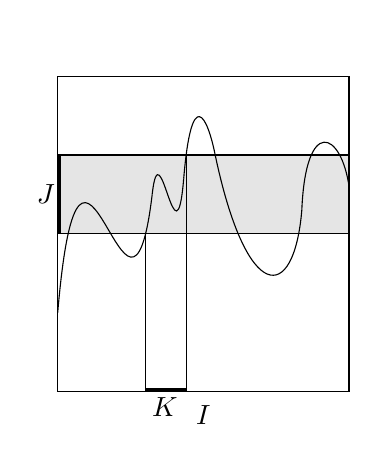
\begin{tikzpicture} 
	\filldraw[fill=gray!20] (0,-0.5) rectangle (3.7, 0.5);
	\Bezier{0,-1.5}{0.3,2}{0.9,-2.5}{1.2,0}
	\Bezier{1.2,0}{1.3,0.9}{1.5,-1}{1.6,0.2}
	\Bezier{1.6,0.2}{1.7,1.4}{1.9,1}{2,0.5}
	\Bezier{2,0.5}{2.4,-1.4}{3,-1.4}{3.1,-0.2}
	\Bezier{3.1,-0.2}{3.15,1}{3.6,0.8}{3.7,0.1}
	\draw (0,-2.5) rectangle (3.7, 1.5);
	\draw (1.115,-2.5) -- (1.115,-0.5);
	\draw (1.63,-2.5) -- (1.63,0.5);
	\draw[line width=1.2] (0.02,-0.5) -- (0.02,0.5);
	\draw[line width=1.2] (1.115,-2.48) -- (1.63,-2.48);
	\node (K) at (1.36, -2.7) {$K$};
	\node (J) at (-0.15, 0) {$J$};
	\node (I) at (1.85, -2.8) {$I$};
\end{tikzpicture}

\end{document}